
System security metrics are valuable only if they can produce timely, actionable measurements. In this thesis we have demonstrated a path forward for developing, testing, validating, and integrating security metrics into the full life cycle of a system. 

In Chapter \ref{ch:background} we present the current state of security metrics. We list the working taxonomies that these metrics can be categorized by, and elaborate on the distinctions that lead to confusion when discussing security measurements. We then review modeling techniques and how these models can isolate the security properties of a system we intend to measure. 

Chapter \ref{ch:automation} presents our unified framework for security measurement and analysis, including the model for implementing individual metrics and the infrastructure built around these metrics to drive automation in a variety of scenarios. Here we establish the security metric inheritance hierarchy and enumerate properties common to all metric types and those specific to each metric subtype. We provide our extensions to attack models that expand the range of systems that can be represented. We describe how we implemented automation from the view points of a security researcher or measurement analyst, and develop our concept of security metrics as a service, \textit{S-MaaS}, with considerations for deployment in a continuous integration or stream processing environment.

Chapter \ref{ch:benchmarking} develops our solution to the lack of validation in the field of security metrics. We establish a set of validation criteria that are needed for acceptance of any metric. We define a fixed set of models that set a frame of reference for evaluating security metrics, and explain how these models can be used to isolate key properties of interest. We investigate the instrumentation needed to validate our metrics in a general manner, and implement this validation framework as extensions to an industry accepted benchmarking tool to maximize the audience and reduce friction to entry. Finally we demonstrate our enhancements built around benchmarking to automate the process of executing tests, analyzing results, and alerting on anomalies and outliers that are uncovered during large scale or long running tests.

Chapter \ref{ch:case_studies} presents a case study conducted as part of AT\&T's planning for infrastructure migration. The study applies the CSAF\cite{Abraham_Nair_2015a} pipeline to hypothetical network architectures and gives insight into how model based security metrics can be used to rank an analysis of competing alternatives. As this study occurred early in the research phase, it had a great impact on the direction this thesis has taken. With the benefit of hindsight we are able to demonstrate both the contributions made during that initial work as well as the progress that has been made since it was completed. 



\begin{figure}[ht]
\centering
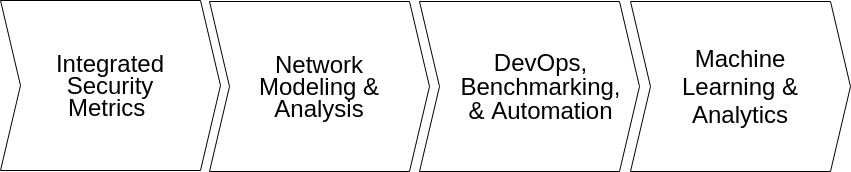
\includegraphics[width=\textwidth]{resource/img/ch_future/timeline_broad.png}
\caption{General Progression and Direction of Thesis}
\label{fig:future:timeline_broad}
\end{figure} 

Figure \ref{fig:future:timeline_broad} captures with broad strokes the path our research has followed and the direction it is heading, while the timeline in Figure \ref{fig:future:timeline_detail} summarizes previous research items that support this thesis. Listed along the top are the two long running projects that have provided both requirements and solutions in this work. SDN Migration Analytics is the focus of the case study in Chapter \ref{ch:case_studies} while the Cloud Benchmarking research has provided an in depth knowledge of designing and validating cyber measurement instruments. Immediately below the long running projects are short term studies conducted over summers each year. The Tactical Edge work that bookends the summer research items focused on evaluating the security of non traditional network architectures and drove our requirement to validate metrics outside of the enterprise domains commonly found in the literature. The Maru research over the summer of 2017 and 2018 led to the development of a distributed streaming analytics system run from within a hardware trusted enclave, which forms the basis of the S-MaaS architecture described in \ref{sec:smaas:arch}. On the right side a legend designates presentations, posters, and papers delivered that relate to the research topics listed above.


\begin{figure}[ht]
\centering
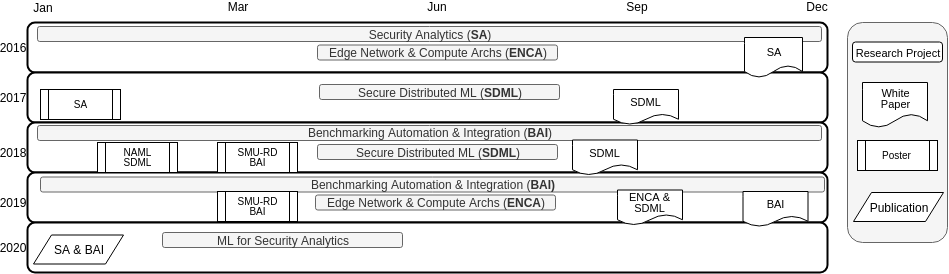
\includegraphics[width=\textwidth]{resource/img/ch_future/timeline.png}
\caption{Timeline of Work Supporting Thesis }
\label{fig:future:timeline_detail}
\end{figure} 

% The timeline in Figure \ref{fig:future:furure_work} identifies critical degree requirement milestones along the top and anticipated deliverables along the bottom. 

% Currently we are preparing submissions, adding models and collecting evidence for the metric validation work, and plan to submit that around the same time as qualifying exams. We are able to create the labeled datasets for the ML models as part of the validation work, and can begin training once the datasets are created. As we discussed in Chapter \ref{ch:future}, the applications of ML in cyber security are limited in scope to a small set of applications like traffic classification for intrusion detection and flow analysis for DDoS prevention. Nothing we found in the review of the literature considered system or threat topology when applying ML.a  We feel confident that our work creates novel datasets that will lead to interesting and valuable results in applied learning techniques. 